\chapter{Device Background}\label{cha:device_background}

Before describing measurements at the focus of this thesis, it is important to first introduce the devices used to engineer interesting states, and the tools used to measure them. As an overview, the chip is made of a material called GaAs/AlGaAs heterostructure, the precise layering of the semiconductors form a two dimensional electron gas (2DEG) around 50\,-\qty{100}{nm} below the surface of the heterostructure. Voltages applied to patterned metallic gates ontop of the heterostructre tune the potential landscape in the 2DEG, this controls where the electrons can go. This tunability allows for the formation of quantum structures such as quantum point contacts (QPCs) and quantum dots (QDs). Ohmics are used to contact the 2DEG, allowing for transport measurements through such structures. 



\section{Two Dimensional Electron Gas (2DEG)}



\begin{figure}[!htb]
  \begin{center}
%% psfrag: comment the following line if not using the psfrag package
    % \psfrag{pie makes me happy!}{$\pi$ makes me happy!}
%% includegraphics: comment the following if not using the graphicx package
    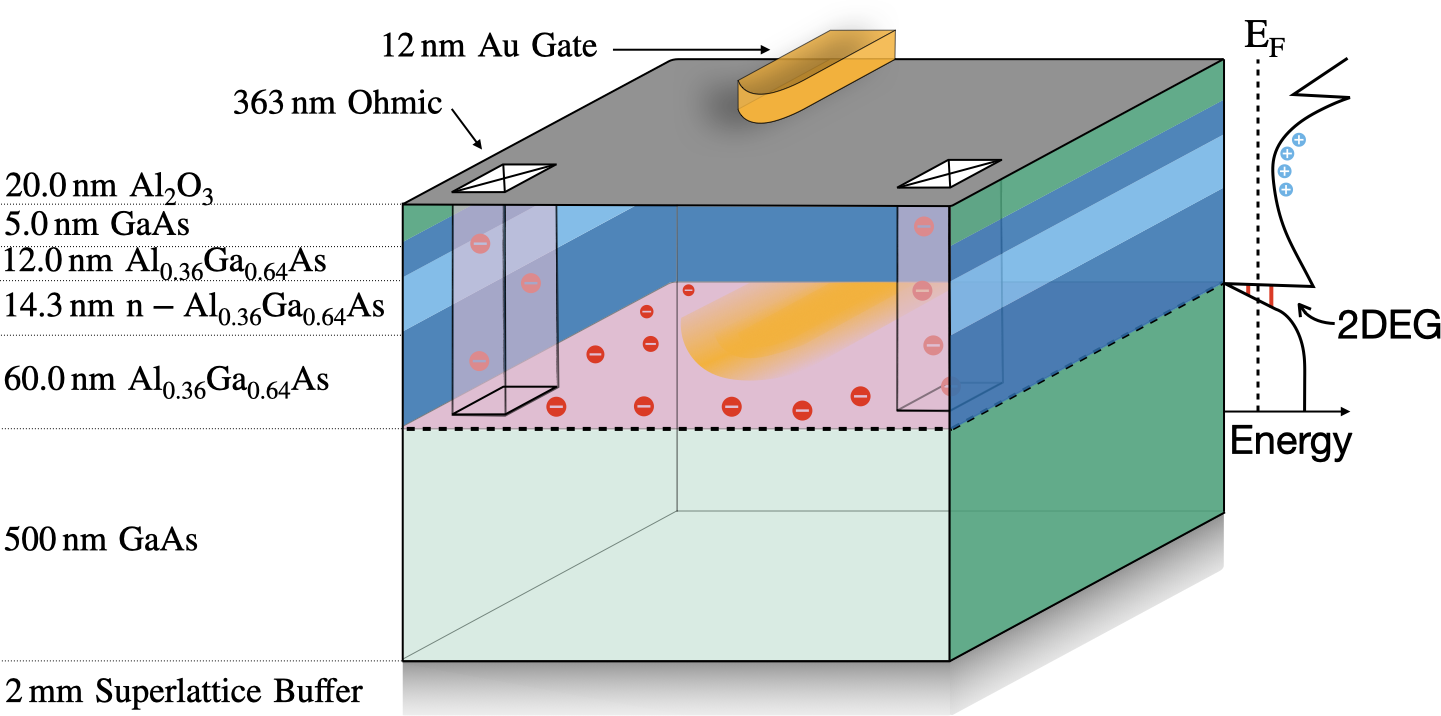
\includegraphics[width=1.0\textwidth]{figures/ch1/crop_FiguresMaster.002.png}
    \caption[Two dimensional electron gas in a GaAs/AlGaAs heterostructure]{\label{fig:ch1/2deg} 
    % For some options that work with pdf\LaTeX, please see this discussion:
    %   \url{http://tex.stackexchange.com/questions/11839}.  
    Illustration of a GaAs/AlGaAs heterostructure with the addition of ohmics and gates used to measure conductance and engineer quantum dots respectively. At the boundary between GaAs and AlGaAs, a two dimensional electron gas (2DEG) is formed. A 2DEG can be thought of as a two dimensional plane of electrons which can move freely along the x and y direction, but are tightly confined in the z direction. Ohmics are made by annealing Ni-Au-Ge, the metal diffuses through the heterostructure making contact to the 2DEG. Gates are used to control the potential in the 2DEG. Negative (positive) voltage on the gates repel (attract) the electrons.
      }
  \end{center}
\end{figure}



The quantum point contacts (QPCs) and quantum dots (QDs) described later in this thesis are engineered in a two dimensional electron gas (2DEG). A 2DEG can be thought of as a two dimensional plane of electrons. The electrons can move freely along the x and y direction, but are tightly confined in the z direction. The 2DEGs' in this thesis are realised in GaAs/AlGaAs heterostructures Fig.~\ref{fig:ch1/2deg}. A semiconductor heterostructure refers to a material system, composed of two or more semiconductor materials with different bandgaps or lattice constants, that are layered together. These layers are typically grown on top of each other using techniques such as molecular beam epitaxy (MBE). The heterostructures in this thesis are grown by Michael Manfra's lab at Purdue University~\cite{manfra_high_quality}. 

There are two characteristics of this heterostructure which give rise to a 2DEG. Firstly, $\mathrm{Al_xGa_{1-x}As}$ has a tunable bandgap ranging from 1.42 - \qty{2.16}{eV}~\cite{gaas_overview} whilst GaAs has a bandgap of \qty{1.42}{eV}. Secondly, an n type dopant layer is sandwiched between the $\mathrm{Al_xGa_{1-x}As}$ layers~\cite{dopant_layer}. The smaller bandgap of GaAs allows the electrons from the donar atoms in the dopant layer to drop into the GaAs conduction band, resulting in a triangular potential well Fig.~\ref{fig:ch1/2deg}. This triangular well contains multiple energy levels. However, the second energy level is $\qty{\sim 150}{meV}$ above the first and will remain unoccupied as the energy gap is much greater than measurement temperatures $\qty{500}{mK}\sim\qty{43}{\mu eV}$ and source drain bias $\qty{100}{\mu eV}$, hence, the electron gas is considered two dimensional~\cite{BEENAKKER_1991}.

Efforts are made to keep the heterostructure and 2DEG clean and defect free. A \qty{7}{nm} cap of GaAs is placed ontop of the heterostructure to prevent oxidation. Also, a small lattice mis match between the GaAs and AlGaAs~\cite{gaas_superlattice} layers keeps the number of boundary defects in the 2DEG plane low. The \qty{30}{nm} AlGaAs buffer layer between the 2DEG and dopants helps prevent defects near the 2DEG plane. The resulting 2DEGs' has a high mobility $\mathrm{\mu_e}~=~\qty{2.56e6}{cm^2/Vs}$ and electron density $\mathrm{n}~=~\qty{2.42e11}{cm^{-2}}$

Fabrication details on these devices is described in Appendix~\ref{cha:appendix1}. As an overview, the heterostructure is divided into separate areas with isolated 2DEGs' by etching away the top layers of the heterostructure to remove the 2DEG underneath. Contact to the 2DEG is made with ohmics contacts. These are made by annealing a layer of Ni-Au-Ge, the metal diffuses through the heterostructure and forms an electrical connection to the 2DEG. Ontop of that, an insulating dielectric of \qty{10}{nm} $\mathrm{Al_2O_3}$ is deposited across the surface of the heterostructure to limit leakage from the metallic gates~\cite{insulating_gates} that are added afterwards. A thin layer (\qty{10}{nm}) of Au is deposited to form the inner gates. The structure and shape of the inner gates have been carefully designed so that QPCs and QDs can be formed in the 2DEG. In a second step, a thick layer (\qty{100}{nm}) of Au is deposited (our outer gates) to connect the inner gates to square bond pads. Wire bonds are then made from a chip carrier to the square bond pads on the chip, so that connection can be made between fridge wiring and the quantum device. 




\afterpage{\clearpage}
\section{Quantum Point Contact (QPC)}

\begin{figure}[!htb]
  \begin{center}
%% includegraphics: comment the following if not using the graphicx package
    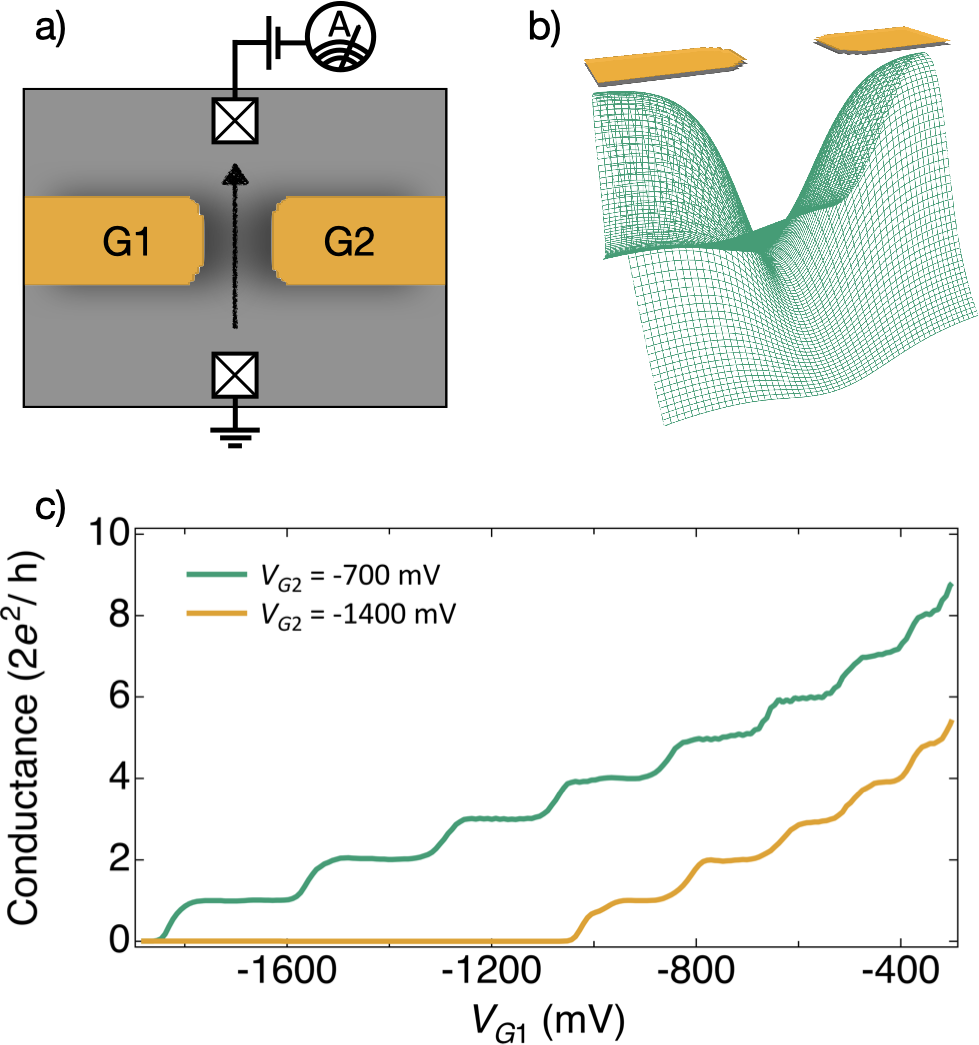
\includegraphics[width=0.85\textwidth]{figures/ch1/crop_FiguresMaster.003.png}
    \caption[Conductance through a quantum point contact]{\label{fig:ch1/qpc_intro} 
    % For some options that work with pdf\LaTeX, please see this discussion:
    %   \url{http://tex.stackexchange.com/questions/11839}.  
    (\textbf{a}) A graphic representation from a top down view of a quantum point contact (QPC). The gold fingers are the metallic gates where negative voltages can be applied to. The grey is where the electrons in the 2DEG can go, dependant on the amount of negative voltage applied to the gates. The crossed squares are ohmic contacts to the 2DEG. These contacts allow a bias across the QPC to be applied, so a conductance through the QPC can be measured. (\textbf{b}) Is a representation of the electric potential the electrons see in the 2DEG due to negative voltage applied to the gates. With sufficient negative voltages applied to the gates, the electrons cannot overcome the potential barrier under the gate and flow between the gates. (\textbf{c}) Is a measurement showing the quantised conductance through a QPC, as the voltage on G1 becomes more negative. At sufficiently negative voltages, the potential barrier between the gates is large enough that a measurement will not see any tunneling events and the conductance is effectively zero. The pinch off is shifted from a more negative (green) to a less negative (yellow) value by increasing the negative voltage applied to G2.
      }
  \end{center}
\end{figure}

In this thesis, a quantum point contact (QPC) is one dimensional channel connected to a source and drain reservoir Fig.~\ref{fig:ch1/qpc_intro}. Such a one dimensional channel in the 2DEG can be engineered by applying sufficient negative voltage on two metal gates on the surface of the heterostructure with a gap in between. Using the ohmics, a potential bias can be applied across the QPC and a current will flow. The more negative the voltage on the gate, the higher the potential barrier is for the electrons in the 2DEG. A large enough potential barrier can stop the electrons flowing underneath the gate (called 'depletion'). However, due to the gap between the gates the electrons can still flow from one side of the QPC to the other Fig.~\ref{fig:ch1/qpc_intro}\textbf{b}. It normally requires a more negative voltage to stop electrons flowing between the gates (called 'pinch off'). A QPC length is the length of the one dimensional channel and the width is the empty space between gates. In the devices used in this thesis, a QPC can have lengths 50~-~\qty{350}{nm} and widths 100~-~\qty{350}{nm} depending on it usage.

The electrons are free to move in the y direction, but if the width of the QPC is comparable to the Fermi wavelength, the allowed energy levels are quantised in the x direction. The confining potential in the x direction can be modelled as a parabolic potential. Hence, allowed 1d energy levels will resemble solutions to the harmonic oscillator Fig.~\ref{fig:ch1/qpc_intro}\textbf{b}. In the absence of a magnetic field, each occupied energy level contributes $\mathrm{2e^2/h}$ to the conductance. The $2$ comes from the spin degeneracy of the electrons, which can be lifted with magnetic field. When measuring the conductance through a QPC as it is pinched off Fig.~\ref{fig:ch1/qpc_intro}\textbf{c}, a signature of the quantised conductance are plateaus at integer values of $\mathrm{2e^2/h}$~\cite{qpc_first_measurement}. At zero temperature, the steps between plateaus would resemble sharp step functions. However, this is smeared out by temperature in a real measurement.

In our devices, QPCs are utilised to form tunable tunnel barriers between a quantum dot and a reservoir (described in the next section) and charge sensors~\cite{cs_first_measurement} which are used to measure the charge around a quantum dot. 




\afterpage{\clearpage}
\section{Quantum Dot (QD)}

\begin{figure}[!htb]
  \begin{center}
%% includegraphics: comment the following if not using the graphicx package
    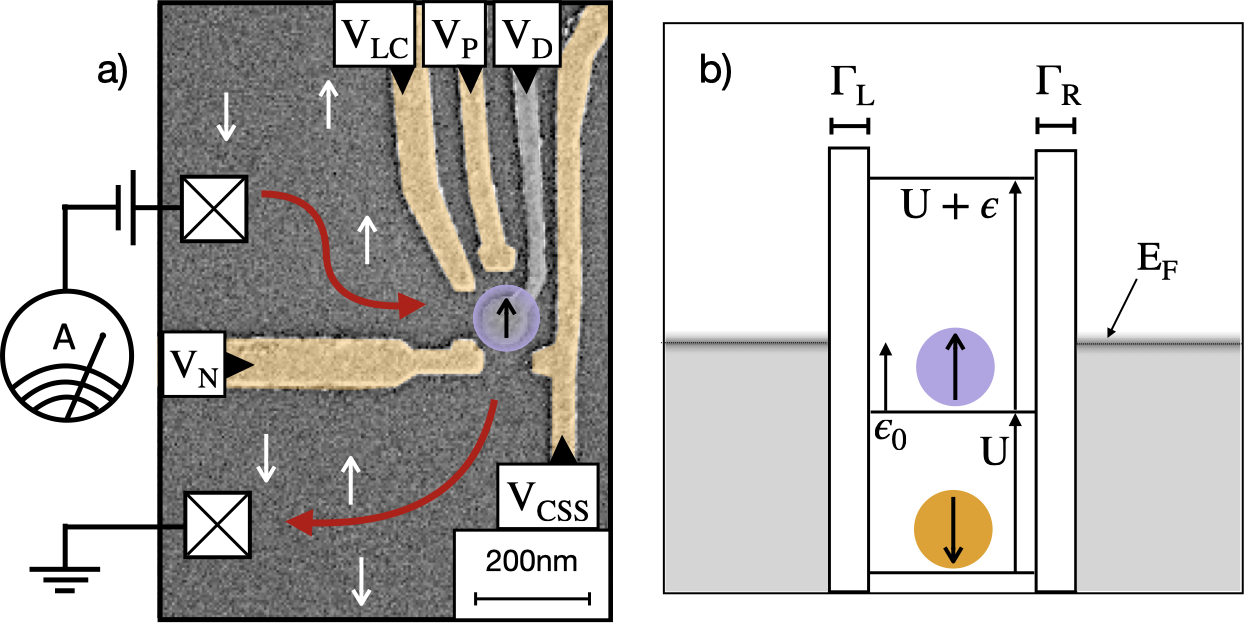
\includegraphics[width=0.9\textwidth]{figures/ch1/crop_FiguresMaster.004.png}
    \caption[Quantum dot energy levels]{\label{fig:ch1/dot_energy_levels} 
    % For some options that work with pdf\LaTeX, please see this discussion:
    %   \url{http://tex.stackexchange.com/questions/11839}.  
    (\textbf{a}) An SEM image of the gates used to define a quantum dot. The gold coloured gates indicate sufficient negative potential is applied such that the 2DEG below is depleted. The gates V\textsubscript{P} or V\textsubscript{D} have the largest effect on dot energy $\epsilon_0$ without changing other energies. The crossed squares are ohmic contacts which contact the 2DEG. By applying a small bias to the ohmics, conductance through the quantum dot is measured. (\textbf{b}) Is a Coulomb blockade energy diagram. The grey boxes represent continuous energy levels of the electrons in the leads. The white rectangles represent tunnel barriers into and out of the quantum dot. The rate of tunneling is denoted by the parameter $\Gamma$, the wider (narrower) the barrier, the smaller (larger) the rate of tunneling. The orange circle represent the first electron in the quantum dot with spin down. The second electron (purple) will pair with the first spin down electron, so the energy required to add the second electron is the charging energy $\mathrm{U}$. To add the third electron (not currently in the quantum dot), the charging energy $\mathrm{U}$, plus the orbital level spacing energy $\Delta$ is required.}
  \end{center}
\end{figure}


In this thesis, a quantum dot (QD) is zero dimensional structure that is formed by connecting a potential well to source and drain reservoirs through a tunnel barrier~\cite{spins_in_qd}. Similar to a QPC, the potential well is formed by applying negative voltages to gates to confine a small region in the 2DEG Fig.~\ref{fig:ch1/dot_intro}\textbf{a}. The tunnel barriers that connect this isolated region in the 2DEG to source and drain reservoirs, are formed by QPCs. The first characteristic of quantum dots is the charging energy $\mathrm{U}$, this is the energy required to add or remove an electron from the quantum dot due to the Coulomb force. 
Under certain conditions, the charge in the quantum dot is quantised and equal to $\mathrm{Ne}$, where $\mathrm{N}$ is the total number of electrons and $\mathrm{e}$ is the charge of a single electron. The two conditions for quantised charge are $\mathrm{R_t}>>\mathrm{h/e^2}$ and $\mathrm{U}>>\mathrm{k_BT}$. The first condition is the resistance of the tunnel barriers $\mathrm{R_t}$, should be greater than the resistance quantum $\mathrm{h/e^2}=\qty{25.813}{k\Omega}$. Qualitatively, the tunnel barriers should be large enough so the electron is located either in the source or drain leads, or in the quantum dot. The second condition is that the charging energy $\mathrm{U}$, should be larger than the thermal energy of the system. These conditions lead to quantised charge in the quantum dot. However, quantised charge is not a unique feature of quantum dots as it has been seen in small metallic islands such as Sn particles~\cite{first_quantised_charge} or nanowires~\cite{nanowire_quantisedcharge}.
The second characteristic of a quantum dot, is if the size of the dot is comparable to the deBroglie wavelength. If this criteria is matched, there are additional contributions to the energy level spacing from the orbital level spacing~\cite{Kouwenhoven_1997_electron_transport}. Take an example 1d box of size $\mathrm{L}$, the orbital level spacing is $\mathrm{\Delta}=(\mathrm{N}/4)\hbar^2\pi^2 / \mathrm{m^*L^2}$, where $\mathrm{m^*}=0.67\mathrm{m_e}$ is the effective mass of electrons. Similar to the emergence of quantisation of charge in the quantum dot when appropriate conditions are satisfied. Contributions from orbital level spacing are important when $\mathrm{\Delta}>>\mathrm{k_BT}$ where the energy level spacing is greater than the thermal energy of the system. 

\afterpage{\clearpage}
\subsection{Conductance Through a Quantum Dot}


\begin{figure}[!htb]
  \begin{center}
%% includegraphics: comment the following if not using the graphicx package
    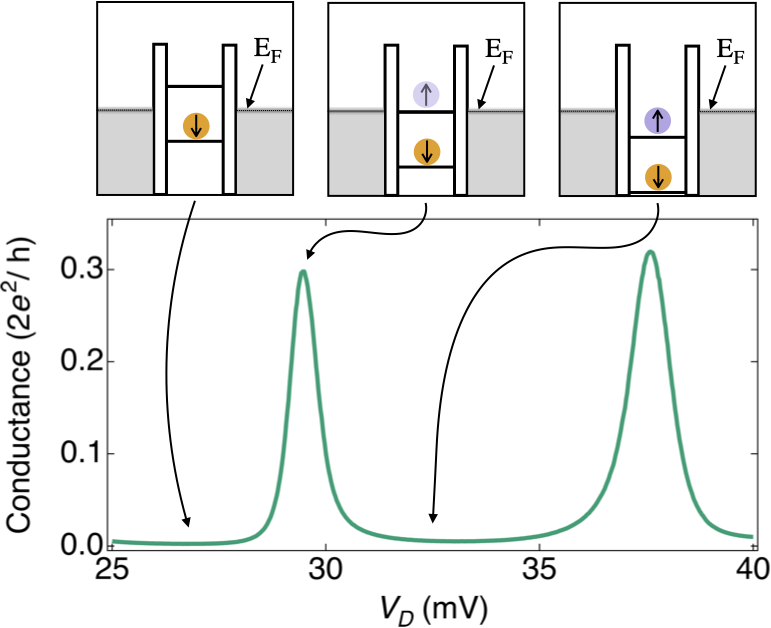
\includegraphics[width=0.85\textwidth]{figures/ch1/crop_FiguresMaster.005.png}
    \caption[Conductance through a quantum dot]{\label{fig:ch1/dot_intro} Measured conductance through a quantum dot (green trace) as a single electron is added and the corresponding Coulomb blockade energy diagrams, showing how the energy levels vary. In 1) there is a single electron in the quantum dot (orange dot). The next available energy level is empty as it above the Fermi energy of the source and drain leads. The conductance is zero as no electron in the leads has sufficient energy to tunnel into the quantum dot. In 2) V\textsubscript{D} is made more positive which lowers the dot energy $\epsilon_0$. The dot energy is now in line with the Fermi energy of the source and drain leads. Resonant tunneling through the quantum dot shows up as a maximum in measured conductance. On average, there is a fraction of the electron charge in the quantum dot (partial purple dot). In 3) the V\textsubscript{D} is made more positive and the dot energy $\epsilon_0$ is below the thermal broadening of the electrons in the source and drain leads. The quantum dot is fully occupied (purple dot) and conductance drops to zero.

      }
  \end{center}
\end{figure}


A quantum dot is formed by applying negative voltages to confine a small region in the 2DEG Fig.~\ref{fig:ch1/dot_intro}\textbf{a}.
Each of the gates near the quantum dot are capacitively coupled to parameters that determine different energies in the dot. 
Careful gate design was used so that each gate has a primary function e.g. varying the tunnel barrier or potential well depth. In Fig.~\ref{fig:ch1/dot_intro}\textbf{a}, $\mathrm{V_{LC}}$ is the 'left coupling' gate and has the strongest effect on the left tunnel barrier along with $\mathrm{V_{N}}$. $\mathrm{V_{N}}$ is the 'nose' gate and effects both couplings equally, it also has a large effect on the dot energy and can push the location of the electron wave function closer to $\mathrm{V_{CSS}}$. $\mathrm{V_{CSS}}$ is the 'charge sensor spine', the charge sensor is discussed in the next section, but it is important for the wavefunction of the electron to be close to $\mathrm{V_{CSS}}$ for higher sensitivity of the charge sensor. $\mathrm{V_{P}}$ is the 'plunger' and is used primarily to control the dot energy $\epsilon_0$ as it is far from the tunnel barriers. By making this gate less negative the dot energy decreases or the size of the potential well increases and at some point, another electron can enter the quantum dot. $\mathrm{V_{D}}$ is the 'dot' gate, this gate is operated different to the other gates as it lies above where the dot lives. This gate is most strongly coupled to the dot energy and is used to add or remove single electrons into the quantum dot with fine control. This gate is normally at positive voltage values to help form a nicely shaped potential well, as negative voltages will form a donut shaped potential. 





\afterpage{\clearpage}
\subsection{Charge Sensing a Quantum Dot}


A charge sensor is a way to measure changes in the charge around the quantum dot. If correctly tuned, it is very sensitive to the additional charge of an electron that enters a quantum dot. It is formed by adding a QPC in close proximity to the quantum dot Fig.~\ref{fig:ch1/dot_intro}\textbf{a}. 

\begin{figure}[!htb]
  \begin{center}
%% includegraphics: comment the following if not using the graphicx package
    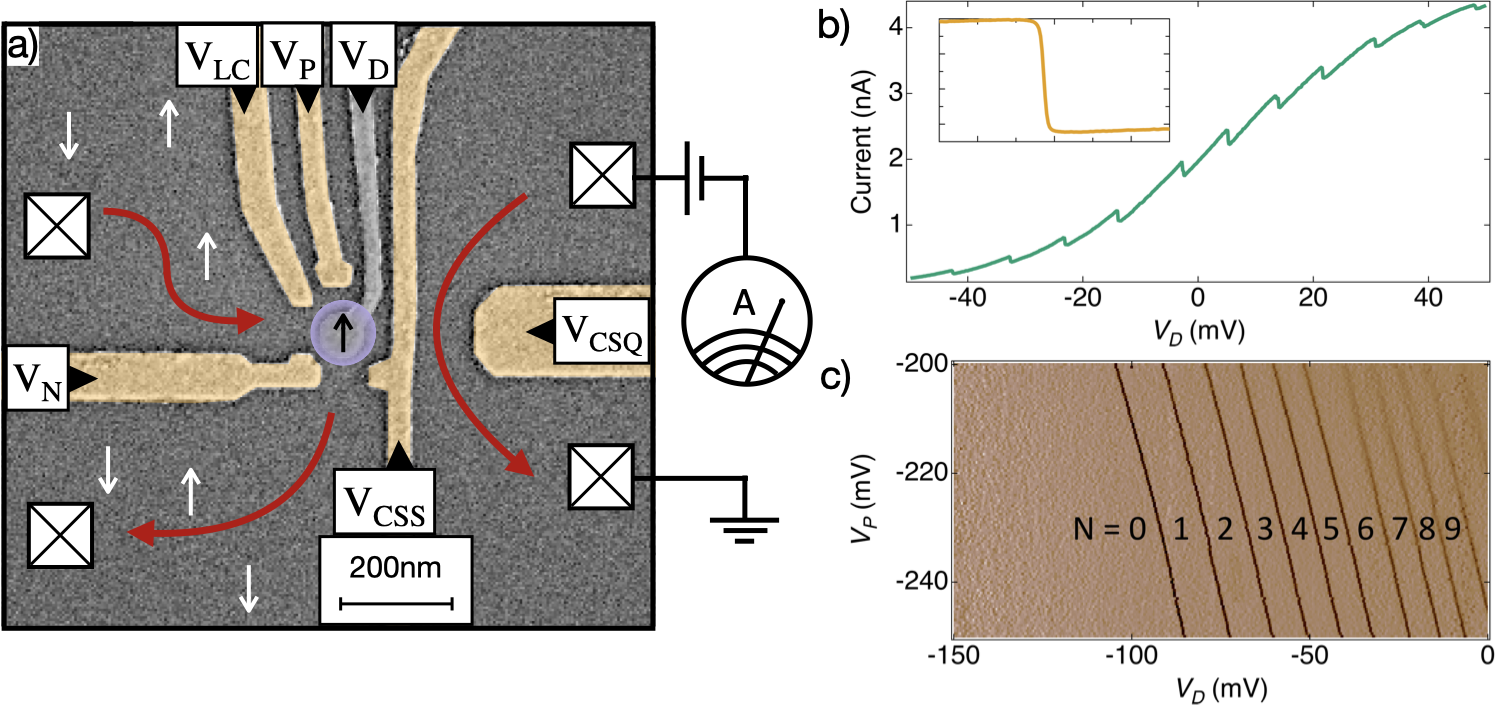
\includegraphics[width=0.95\textwidth]{figures/ch1/crop_FiguresMaster.006.png}
    \caption[Charge sensing a quantum dot]{\label{fig:ch1/ct_intro} 
    % For some options that work with pdf\LaTeX, please see this discussion:
    %   \url{http://tex.stackexchange.com/questions/11839}.  
    (\textbf{a}) An SEM image of the gates used to define a quantum dot. The gold coloured gates indicate sufficient negative potential is applied so that the 2DEG below is depleted. The gates V\textsubscript{P} or V\textsubscript{D} have the largest effect on dot energy $\epsilon_0$ without changing other energies. The crossed squares are ohmic contacts which contact the 2DEG. V\textsubscript{CSQ} is used to form a QPC near the quantum dot. By setting up the QPC on a steep slope in between conductance plateaus, the current through the QPC is sensitive to nearby changes in charge. (\textbf{b}) Measuring the current across the charge sensing QPC. As V\textsubscript{D} becomes less negative the current through the QPC increases. The downward jumps in current are a result of the negative repulsion from electrons entering the quantum dot (called charge transitions). The inset (yellow) shows a zoomed in scan over one of these transitions. (\textbf{c}) A 2d map showing how the occupation of the quantum dot changes as a function of V\textsubscript{P} and V\textsubscript{D}. The data is the differentiated current through the charge sensor. The differential of the steep slopes in a charge transition show up as sharp peak. This is useful for locating charge transitions when there is a large change in background current. 
      }
  \end{center}
\end{figure}


By changing the voltage applied to a gate, a QPC can be tuned so that the current is on a steep slope or plateau Fig.~\ref{fig:ch1/qpc_intro}\textbf{c}. When used as a charge sensor, the QPC is adjusted to be on a steep slope. In this setting, small changes in nearby potentials (x axis of a QPC trace) show up as large changes in the current measured through the QPC~\cite{cs_design}. In Fig.~\ref{fig:ch1/dot_intro}\textbf{b}, the QPC is set up on a steep slope and V\textsubscript{D} is swept from negative to positive, lowering the dot energy $\epsilon_0$ past the Fermi energy of the leads, so that an electron can tunnel into the dot. The background increase in current is due to the capacitive coupling of V\textsubscript{D}. As V\textsubscript{D} is swept to more positive voltages, the potential in the QPC lowers and the measured current increases. Once an electron can tunnel into the quantum dot, the extra negative charge of the electron shows up as a small, but sharp decrease in current through the QPC, which is called a 'charge transition'. The derivative of the current can be used to identify charge transitions in large scans where there is a large change in background current. The steep slope of the charge transition shows up as a large negative spike in the derivative. 

One of the functions of the charge sensor is to count how many electrons are in the quantum dot Fig.~\ref{fig:ch1/dot_intro}\textbf{c}. By making V\textsubscript{D} more negative and ensuring the tunnel barriers are small enough for electrons to enter the quantum dot, at some point there will be a final charge transition signalling the last electron. A 2d sweep with different gates on either axis reveals the relative cross capacitance between each gate on the dot energy $\epsilon_0$. From Fig.~\ref{fig:ch1/dot_intro}\textbf{c}, a \qty{-50}{mV} change on V\textsubscript{D} removes $\sim~4$ electrons, but \qty{-50}{mV} change on V\textsubscript{P} only removes $\sim~2$ electrons.



% \afterpage{\clearpage}
\section{Electron Temperature from Charge Transitions}



Charge transitions can be used to count the number of electrons in a quantum dot~\cite{electron_counting}, or determine the relative cross capacitance between different gates on the dot energy.

\begin{figure}[!htb]
  \begin{center}
%% includegraphics: comment the following if not using the graphicx package
    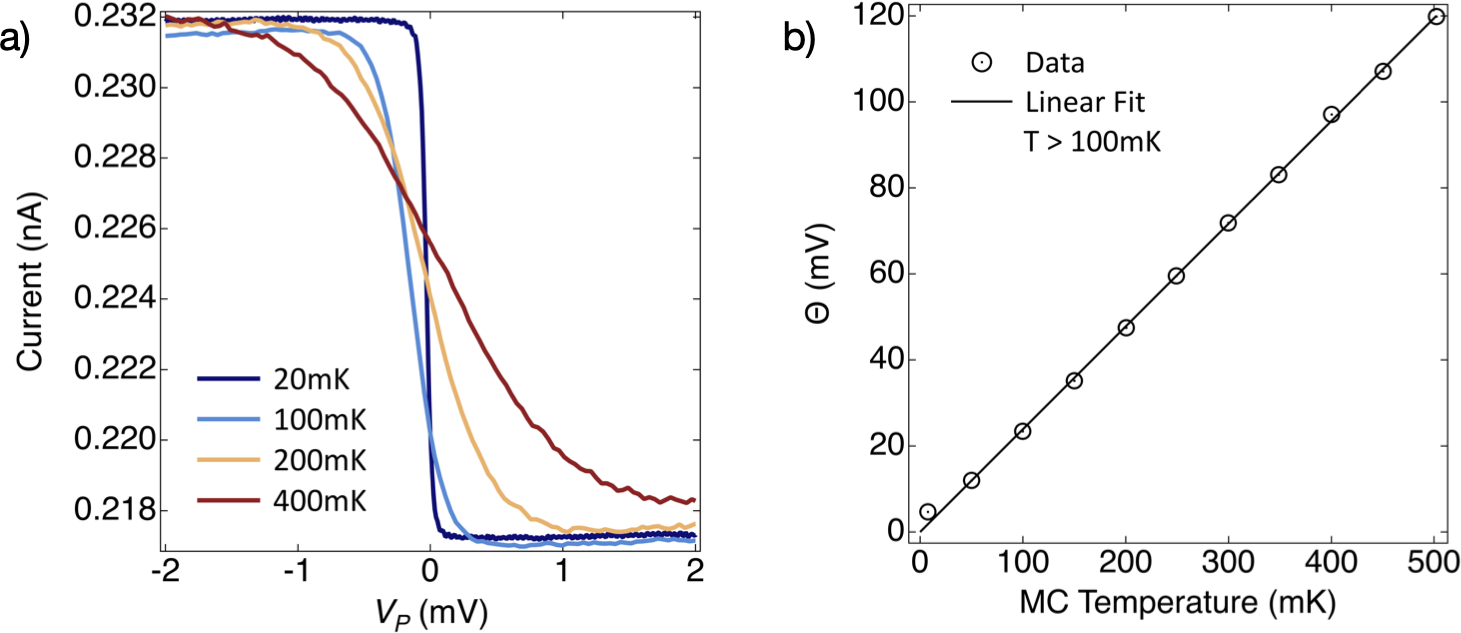
\includegraphics[width=1.0\textwidth]{figures/ch1/crop_FiguresMaster.007.png}
    \caption[Calculating the electron temperature]{\label{fig:ch1/electron_temp} 
    % For some options that work with pdf\LaTeX, please see this discussion:
    %   \url{http://tex.stackexchange.com/questions/11839}.  
    (\textbf{a}) A weakly coupled (thermally broadened) charge transition is measured at different fridge temperatures. The broadening of a weakly coupled charge transition is linearly proportional to its temperature. (\textbf{b}) A plot of the calculated broadening ($\Theta$) of the charge transition, at different fridge temperatures. At fridge temperatures \qty{>100}{mK}, the increase in the charge transition broadening is linear with temperature. This indicates the electrons are well thermalised to the fridge. A linear fit to fridge temperatures \qty{>100}{mK} is extrapolated to base temperature to calculate the real temperature of the electrons given the measured broadening. Electron temperature is determined to be \qty{20}{mK}
      }
  \end{center}
\end{figure}



But, it can also be used to measure the temperature the electrons in the 2DEG. The broadening of the charge transition depends on the temperature of the system and size of the tunnel barriers (strength of coupling $\Gamma$). When the coupling strength is less than the thermal energy of the system ($\Gamma/\mathrm{k_BT} << 1$), the broadening of the charge transition depends only on the temperature of the system. In this regime, the charge transition is described as thermally broadened or weakly coupled. The current lineshape of a charge transition in this regime is,


\begin{equation}\label{eq:cs_lineshape}
  \mathrm{I_{CS}} = 
  \mathrm{I_{amp}}
  \tanh
  \left( 
  \frac{\mathrm{V_P - V_{mid}}}{2\Theta}
  \right) + 
  \gamma \mathrm{V_P}
  + \mathrm{I_{const}}
\end{equation}

where $\mathrm{I_{CS}}$ is the current through the charge sensor. $\mathrm{I_{amp}}$ is the amplitude of the charge transition, $\mathrm{V_{P}}$ is the voltage on the sweep gate used to sweep over the charge transition, $\mathrm{V_{mid}}$ is the mid point of the charge transition. $\Theta=\frac{\mathrm{k_B}T}{\mathrm{\alpha e}}$ is the thermal broadening in units of gate voltage, where $\alpha \equiv \frac{\mathrm{d\epsilon_0}}{\mathrm{dV_P}}$ is a leverarm that relates changes in a gate voltage to changes in the dot energy $\epsilon_0$. $\gamma$ is the cross capacitance between the sweep gate and the current through the charge sensor. $\mathrm{I_{const}}$ is a constant current offset.



The broadening of a temperature broadened charge transition can be used to determine the temperature of the electrons in the 2DEG~\cite{cs_measure_temp}, as the broadening is linearly proportional to the temperature ($\Theta\propto\mathrm{T}$) of the electrons Fig.~\ref{fig:ch1/electron_temp}\textbf{a}. At high fridge temperatures, the electrons in the 2DEG are in thermal equilibrium with the fridge. But as the fridge reaches base temperature (\qty{8}{mK}), the electrons in the 2DEG will not be in equilibrium due to poor thermal contact and sources of electrical noise. Furthermore, large source drain biases across the quantum dot can artificially broaden the charge transition (i.e. \qty{1}{\mu eV}~=~\qty{11.6}{mK}). Similarly, charge noise in the dopant layer can shift the charge transition left or right in gate space, leading to artificial broadening. 


To determine the proportionality constant between the broadening and temperature, charge transitions are measured at a range of fridge temperatures from \qty{8}{}~-~\qty{500}{mK}. Each charge transition is measured quickly ($\sim$\qty{0.5}{s}) and repeated many times ($\sim300$). Any traces with large jumps in current near the charge transition ('charge jumps') are thrown out, and the remaining traces are centered and averaged. The quick scans across the charge transition and averaging reduces additional broadening that come from charge motion in the dopant layer. The amount charge motion in the dopant layer scales between $\mathrm{1/f}$ and $\mathrm{1/f^2}$~\cite{charge_noise}. Each charge transition is then fit using Eq.~\ref{eq:cs_lineshape}, and the calculated $\Theta$ is plotted versus the fridge temperature Fig.~\ref{fig:ch1/electron_temp}\textbf{b}. A linear fit to $\Theta$ between \qty{100}{}~-~\qty{500}{mK} determines the proportionality constant. This constant is used to convert the $\Theta$ calculated as base temperature, into the effective temperature of the electrons in the 2DEG. In this fridge, a base electron temperature of \qty{20}{mK} was determined.



\subsection{Charge Sensing with a Virtual Gate}

\begin{figure}[!htb]
  \begin{center}
%% includegraphics: comment the following if not using the graphicx package
    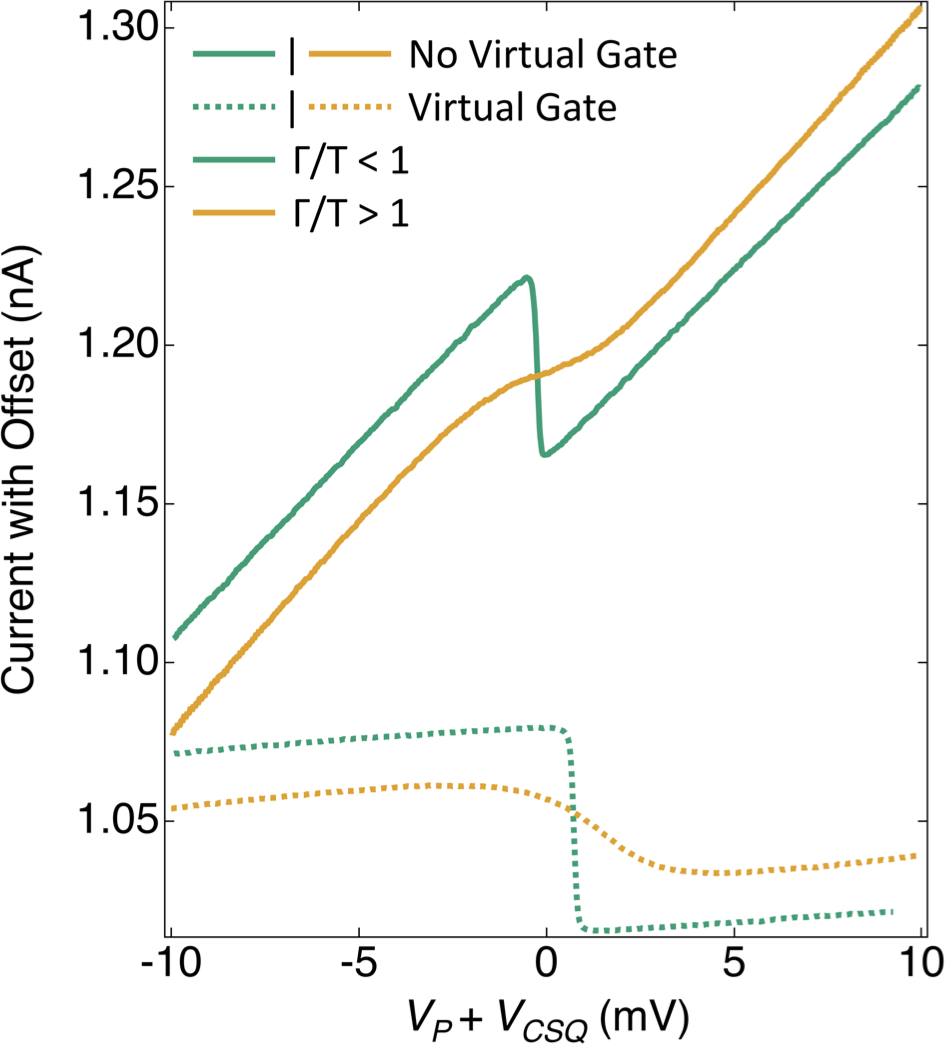
\includegraphics[width=0.8\textwidth]{figures/ch1/crop_FiguresMaster.012.png}
    \caption[Measuring charge transitions with and without a virtual gate]{\label{fig:ch1/virtual_gate_example} 
    % For some options that work with pdf\LaTeX, please see this discussion:
    %   \url{http://tex.stackexchange.com/questions/11839}.  
    Data of a weakly (green) and strongly (yellow) coupled charge transition scanned using a single gate V\textsubscript{P} (solid line) and a virtual gate  V\textsubscript{P}~+~V\textsubscript{CSQ} (dashed line). The traces have been offset in current for clarity. V\textsubscript{P} has a large effect on the dot energy $\epsilon_0$, however, it also changes the current through the charge sensor $\mathrm{I_{CS}}$ due to capacitive coupling. Here, a virtual gate is used to change the dot energy whilst keeping the current through the charge sensor constant. This helps with visually identifying strongly coupled charge transitions which become very broadened. More importantly, the charge sensor stays in the linear regime where changes in the potential are linearly proportional to changes in the current. Note the x axis is only showing the value of V\textsubscript{P}. As V\textsubscript{P} is swept negative to positive, V\textsubscript{CSQ} is swept positive to negative.}
  \end{center}
\end{figure}


Temperature broadened transitions are straightforward to measure and fit. The current lineshape is described by an analytic function, where the broadening depends on a single parameter and the sharpness of the transition, makes visual inspection of the fit trivial. However, the work in this thesis focuses on the gamma broadened regime or strong coupling regime where $\Gamma/\mathrm{k_BT}>1$. The charge transitions in this regime become very spread out and it can be tricky to visually inspect the quality of fit. 

One way to tackle this problem is by using a virtual gate. In general, a virtual gate is a name give to a combination of gates that when varied, change a specific parameter of the quantum dot whilst keeping other parameters constant. The main parameters to control are the dot energy $\mathrm{\epsilon_0}$, left coupling $\mathrm{\Gamma_L}$, right coupling $\mathrm{\Gamma_R}$ and current through the charge sensor $\mathrm{I_{CS}}$. An example usage would be a virtual gate that controls the left coupling $\mathrm{\Gamma_L}$ only. For this specific virtual gate, a combination of V\textsubscript{LC} and V\textsubscript{P} would be used. V\textsubscript{LC} to primarily changed the left coupling $\mathrm{\Gamma_L}$ and V\textsubscript{P} to offset any changes to the dot energy $\epsilon_0$. 


In the context of this thesis, only a single type of virtual gate is used. One that changes the dot energy $\epsilon_0$, but keeps the current through the charge sensor $\mathrm{I_{CS}}$, constant. Fig.~\ref{fig:ch1/virtual_gate_example} shows the effect of this virtual gate on a weakly coupled ($\Gamma/\mathrm{k_BT}<1$) and strongly coupled ($\Gamma/\mathrm{k_BT}>1$) charge transition. Only two gates are used to form this virtual gate, V\textsubscript{P} and V\textsubscript{CSQ}. By sweeping V\textsubscript{CSQ} in the opposite direction of V\textsubscript{P}, the cross capacitive effect of V\textsubscript{P} on the charge sensor is largely removed. 


\afterpage{\clearpage}
\section{Measurement Pocedures}

\subsection{Cooldown Bias}
At room temperature, $+$\qty{200}{mV} is applied to each of the gates forming the quantum dot and charge sensor (apart from V\textsubscript{D}). The positive bias repels the postive charge underneath the gates in the dopant layer. Once the device reaches \qty{10}{K}, the dopants are frozen in and an effective potential is seen by the electrons in the 2DEG due to the absence of positive charge. Cooling with bias has two advantages. One, it reduces the charge noise \cite{bias_cooling}. Two, it reduces the amount of negative potential required on the gates. The effective potential from the positive bias is roughly equal to a negative voltage of equal magnitude when the device is cold (i.e. $+$\qty{200}{mV} cooldown bias $\approx$ $-$\qty{200}{mV}). This is useful as the fine gates can 'blow up' (in reality the metal gates will lift off a little from the heterostructure surface) from high voltages, rendering the device un measurable. The fine gates are also sensitive to static discharge, so \qty{1}{M\Omega} of inline resistance is added to all of the gates.   

\subsection{Gate Dividers}
When measuring charge transitions with a virtual gate, fine gate control at large voltages is often required. For example, V\textsubscript{P} may need a voltage of $-$\qty{500}{mV}, but a resolution of \qty{0.001}{mV}. Digital to analog converter (DAC) channels are used to apply the voltage on the gates. The DACs have a range of $\pm$\qty{10}{V}, with 16 bit resolution. This puts a lower bound on the step size of \qty{0.305}{mV} ($\mathrm{\qty{20}{V}/2^{16}}$). To achieve the large voltage range with high resolution, two DACs are connected to the same gate. One DAC channel is used to cover a wide voltage range, whilst the other is used for fine control by adding a voltage divider in line. Voltage dividers between $20$ and $100000$ are commonly used to achieve the required resolution (up to \qty{3}{nV}). All of the voltages in this thesis have been converted to the real voltage applied to the gate (i.e. not the voltage output on the DAC). However, for clarity reasons, only the fine gate may be shown in a figure, even though an additional rough gate is applying a large voltage to the same gate. 













